This section reports on an inter-annotator agreement (IAA) study that was conducted to investigate the annotation of negation cues in texts related to the vaccination debate using the e-Host annotation tool. The purpose of the study was to compare, analyze, and quantify the annotations made by different annotators and to identify sources of disagreement among them. Following the guidelines provided by Morante et al. \cite{morante2011annotation}, each member of the group independently annotated the same corpus of texts. The corpus contained a mix of pro and anti-vaccination opinions from official sources such as the National Health Service UK, as well as independent publications like the National Vaccine Information Center and Natural News. 


\subsection*{Data Annotation}
Following the Morante et.al. \cite{morante2011annotation} Annotation of Negation Cues and their Scope Guideline, we proceeded to annotate negation cues in texts related to the vaccination debate using the \textit{e-Host} annotation tool. The suggested guidelines indicated the possible negation cues and offered examples at the sentence level on how to determine the scope of the negation from stories by Conan Doyle.  The corpus contained texts from official sources such as the National Health Service UK, but also independent publications like the National Vaccine Information Center or Natural News, thus showing both pro and anti-vaccination opinions. 

The annotation guidelines author offered the possible negation cues for each part of speech, as well as instructions on how to separate the negation scope from the rest of the phrase, based on a simple grammatical analysis. This includes reformulating the phrase to test if a part of it belongs to the scope or not. Moreover, there were examples offered regarding non-continuous scopes and special constructions like questions and imperatives. A set of specific rules on the separation of scope given the part of speech that was negated made the process less prone to annotator bias.
Finally, particular constructions with false negations and non-existing scope were provided to avoid expected mistakes.

All annotations were added to our \href{https://github.com/Sergi095/Applied-Text-Mining-VU-Course-2023-}{GitHub Repository}

\subsection*{Inter-Annotator Agreement Analysis}
% ----------------------------------------------
Inter-annotator agreement (IAA) study brings insights into the annotation process by comparing, analyzing, and quantifying the annotations of different people. In our case, each member independently got familiar with the guidelines and proceeded to annotate 12 texts found in the fifth batch. In order to perform the IAA study, everyone shared their annotated files, which were compared in teams as shown in Figure \ref{fig:Pairwise agreement}.

\begin{figure}
  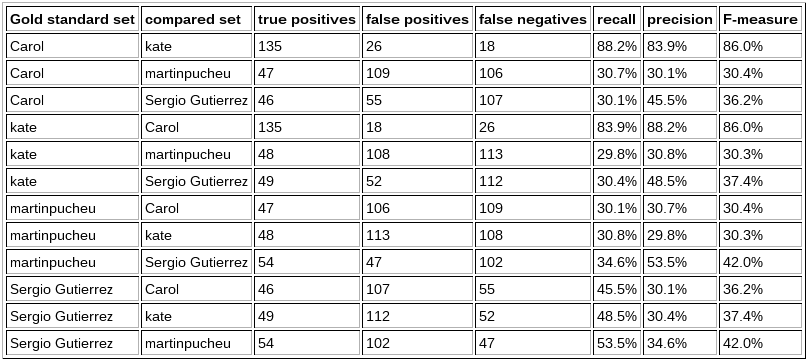
\includegraphics[width=\linewidth]{Plots and results/pairwise.png}
  \caption{Pair-wise agreement}
  \label{fig:Pairwise agreement}
\end{figure}


An error analysis was conducted to systematically identify and explain sources of disagreement among annotators. The analysis was based on a random sample of errors, and patterns were identified and illustrated with examples. The sources of errors were identified as human error and a lack of alignment between the text versions used for annotation. The analysis revealed that most of the annotation differences were caused by these issues, as can be seen in Figures \ref{fig:error2} and \ref{fig:error3}.

To address these issues, it would be beneficial to have a more thorough training process for the annotators and to provide more detailed examples in the guidelines to reduce ambiguity. Additionally, post-processing the annotations to annotate some obvious negations missed by the classifier would also help to improve the overall agreement scores, as shown in Figure \ref{fig:4way}.

\begin{figure}[!h]
\begin{center}
  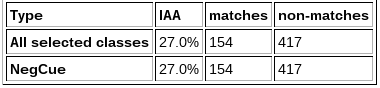
\includegraphics[width=0.6\textwidth]{Plots and results/4way.png}
  \caption{4-way IAA result}
  \label{fig:4way}
\end{center}  
\end{figure}


To sum up, this section describes an inter-annotator agreement (IAA) study that was conducted on a group of annotators who independently annotated a set of texts. This section aimed to bring insights into the annotation process by comparing, analyzing, and quantifying the annotations of different annotators. 

\begin{figure}[!h]
  \includegraphics[width=\linewidth]{images/e1.png}
  \caption{Error example 1}
  \label{fig:error2}
\end{figure}


The process revealed that most of the annotation differences were caused by human error and a lack of alignment between the text versions used for annotation. To address these issues, we suggest implementing a more thorough training process for the annotators and providing more detailed examples in the guidelines to reduce ambiguity. Additionally, post-processing the annotations to annotate some obvious negations missed by the classifier would also help to improve the overall agreement scores.

\begin{figure}[!h]
  \includegraphics[width=\linewidth]{images/e2.png}
  \caption{Error example 2} 
  \label{fig:error3}
\end{figure}


